\section{Extending the Stokes method}

To extend the the previously described mixed finite element method to the general incompressible Navier-Stokes equations,
we must introduce time dependence and advection. We will focus on the Navier-Stokes equations in a closed cavity, with $\rho = 1$, and with zero initial condition and
a no-slip boundary condition everywhere. The equation is then

\begin{equation}\label{navier_stokes_ibvp}
\begin{split}
    \frac{\partial u}{\partial t} + u\cdot\nabla u &= \nu\Delta u - \nabla p + \rho g,\\
    \nabla\cdot u &= 0,\\
    u(\hat{x}, 0) &= 0, \quad \left.u\right|_\Gamma = 0.
\end{split}
\end{equation}

Time dependence is simple. Due to the diffusive nature of the Stokes equation, a viable option for time discretization (to maintain stability) is implicit Euler.
The discretized time-dependent Stokes equations are then
\newcommand{\uprev}{{u_{\text{prev}}}}
\begin{equation}
\begin{split}
    \int_\om \frac{u - \uprev}{\Delta t}\cdot \psi^u\,d\hat{x}
        &= \int_\om \nu \nabla u : \nabla \psi^u - p\nabla\cdot \psi^u + \rho g \cdot \psi^u\,d\hat{x},\\
    \int_\om -\psi^p \nabla\cdot u &= 0 \text{\quad\quad for all $\psi^u \in \Psi^u$ and $\psi^p \in \Psi^p$.}
\end{split}
\end{equation}

The last step is to introduce advection: the term $u\cdot \nabla u$. There are many choices.
\subsubsection{Fully implicit Euler with Newton iterations}
If full implicit Euler is used, and the nonlinear advection term is expanded, the result is a nonlinear system of equations.
The simplest option is then a Newton iteration, solving a sequence of linear systems after computing the Gateaux derivative of the system
at each step. This fully implicit method may be highly accurate, but requires a not-so-straightforward modification of the Stokes flow code.

\subsubsection{A mixed implicit-explicit (IMEX) method}
An alternative method is IMEX, where $u\cdot \nabla u$ is instead $\uprev \cdot \nabla \uprev$ in the implicit Euler step.
This gives a stable implicit momentum diffusion, with a fast, explicit advection step. There are, however, still difficulties in the accurate computation
of $\uprev \cdot \nabla \uprev$ projected onto the P2 finite element space.

\subsection{A splitting method with semi-Lagrangian advection}
The difficulties of the above two methods can be avoided by performing a splitting method.
The essence of the difficulty of solving a fully hyperbolic advection equation lies in the motion of solution data along \textit{characteristic curves}.
The diffusive component of the Navier-Stokes equations, however, makes the system parabolic: there are no well-defined characteristic curves.
If we instead alternate between 
the inertial advective motion of the fluid,
and then apply those non-advective forces (viscosity, body forces, and pressure),
then this first step can use the method of characteristics. The simplest such method is \textit{semi-Lagrangian advection},
which is common in meteorology and computer graphics \cite{stam_stable_fluids}.
The resulting split equations are
\begin{equation}
\begin{split}
    \frac{u^* - \uprev}{\Delta t} &= -\uprev\cdot \nabla\uprev. \\
    \frac{u - u^*}{\Delta t} &= \nu \nabla u -\nabla p + \rho g.
\end{split}
\end{equation}
The second step can be solved with the time-step Stokes flow equation described previously. For the first, advective, step
we can use the method of characteristics. Given that $u$ is sampled at vertices and midpoints in the triangulation, the characteristic curve
at a node $\hat{x}$ is tangent to $u(\hat{x})$. An explicit Euler step will simply ``shift'' the node to $\hat{x} + \Delta t u(\hat{x})$,
with the same velocity (due to inertia).
This is the Lagrangian perspective, and will require either modification of the mesh, or reprojection of the ``shifted''
finite element spaces onto the non-shifted finite element space.
The alternative, \textit{semi}-Lagrangian method, is to sample the velocity \textit{backward} along the characteristic curve,
    $$u(\hat{x}) \leftarrow u(\hat{x} - \Delta t u(\hat{x})).$$
Given the no-slip boundary condition, for small enough $\Delta t$ it seems reasonable to say that
$u(\hat{x} - \Delta t \uprev(\hat{x}))$ is $0$ when $\hat{x} - \Delta t u(\hat{x})$ lies outside of the domain.
The resampling is done with the exact $\uprev$ reconstructed by quadratic basis functions. This can be achieved by either mesh traversal, to locate the triangle
containing $\hat{x} - \Delta t \uprev(\hat{x})$, followed by combination of the quadratic triangle basis functions, or by densely sampling $\uprev$ into
a fine grid, which is used as a lookup table through linear filtering. Given that the domain is 2D, this second option can be done extremely quickly by triangle rasterization (function sampling) on a modern GPU. This avoids the necessity of additional data structures for mesh search.



\section{Results}
I have implemented the semi-Lagrangian method, as described above, by two small extensions
of the Stokes flow method of chapter 5
(timestepping and split semi-Lagrangian advection).
\subsubsection{The sample problem}
As a specific test case, the kinematic viscosity is set to $\nu = 0.001$, and
the domain $\Omega$ is taken as the square with circular obstruction
    $$\Omega = [-1,1]^2 - D,$$
where $D$ is the disk of radius $0.18$ centred at $\hat{x} = (0,0)$.
The initial condition and boundary conditions are the simplest possible: $0$ initial velocity, and no-slip everywhere.
The source function $g$ is what introduces motion into the system. It is defined as
$$
g(\hat{x}) = 
    \left\{\begin{array}{lr}
        (-3000, 0) &\text{if $\hat{x} \in D_g$},\\
        (0, 0) &\text{otherwise},\\
        \end{array}\right.
$$
where $D_g$ is a disk of radius $0.125$ centred at roughly $\hat{x} = (0.85, 0)$.
This emulates a sort of inflow condition at the right-hand-side, without the necessity of handling non-trivial boundary conditions.

\subsubsection{The discretization}
The base square mesh is $60 \times 60$, with velocity sampled at additional midpoints. This mesh, along with the source disk, is
displayed in figure \ref{fig:navier_wireframe}.

\begin{figure}[H]
    \centering
    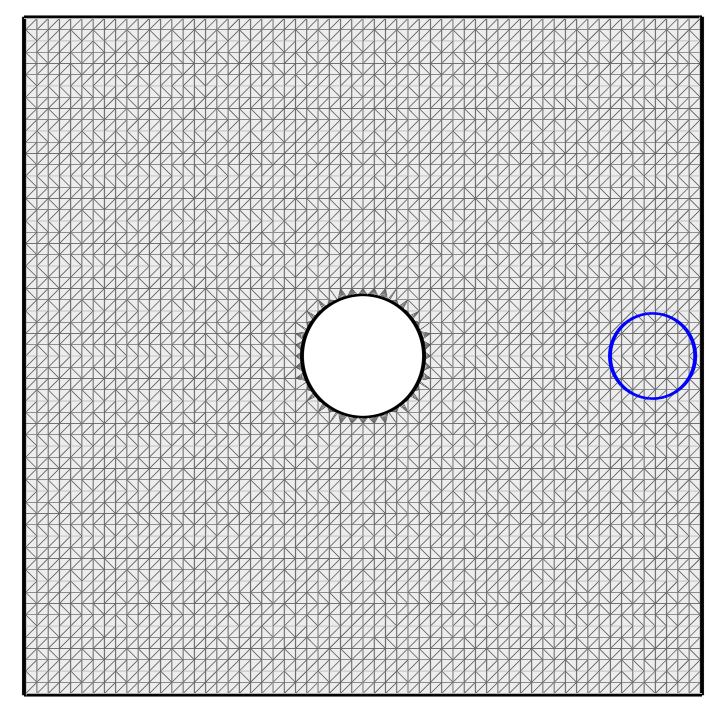
\includegraphics[width=0.4\textwidth]{figures/navier_stokes/wireframe.png}
    \label{fig:navier_wireframe}
\end{figure}

The time step is constant, chosen as $\Delta t = 1/300$. A total of $900$ time steps have been computed, from $t = 0$ to $t = 3$.
This computation took 14 hours on a 2012 laptop, and the code is very unoptimized --- however, the major bottleneck is by far the sparse linear solve. The
advection step is effectively free in comparison (interactive-speed advection versus a minute for the solve on my machine). The resulting sparse matrix is $31895 \times 31895$, with a
fill of approximately $0.0003845/1$.

\subsubsection{Visualisation of the results}
Figures \ref{fig:navier_0} and \ref{fig:navier_1} display the resulting solution at varying times.
The initial flow shown in \ref{fig:navier_0}, as expected, splits symmetrically at the obstruction into two vortices, which then split as they hit the walls.
Subsequently, in figure \ref{fig:navier_1} (which displays a larger range of time steps), symmetry breaks down, the source flow deflects.
The solution past this point cannot be considered as anywhere close to the real solution, due to the onset of turbulence in this medium-Reynolds-number flow. However, important qualitative effects
(for example incompressibility and oppositely-oriented vortices being pushed against the corners of the cavity) are apparent.

\begin{figure}[htbp]
    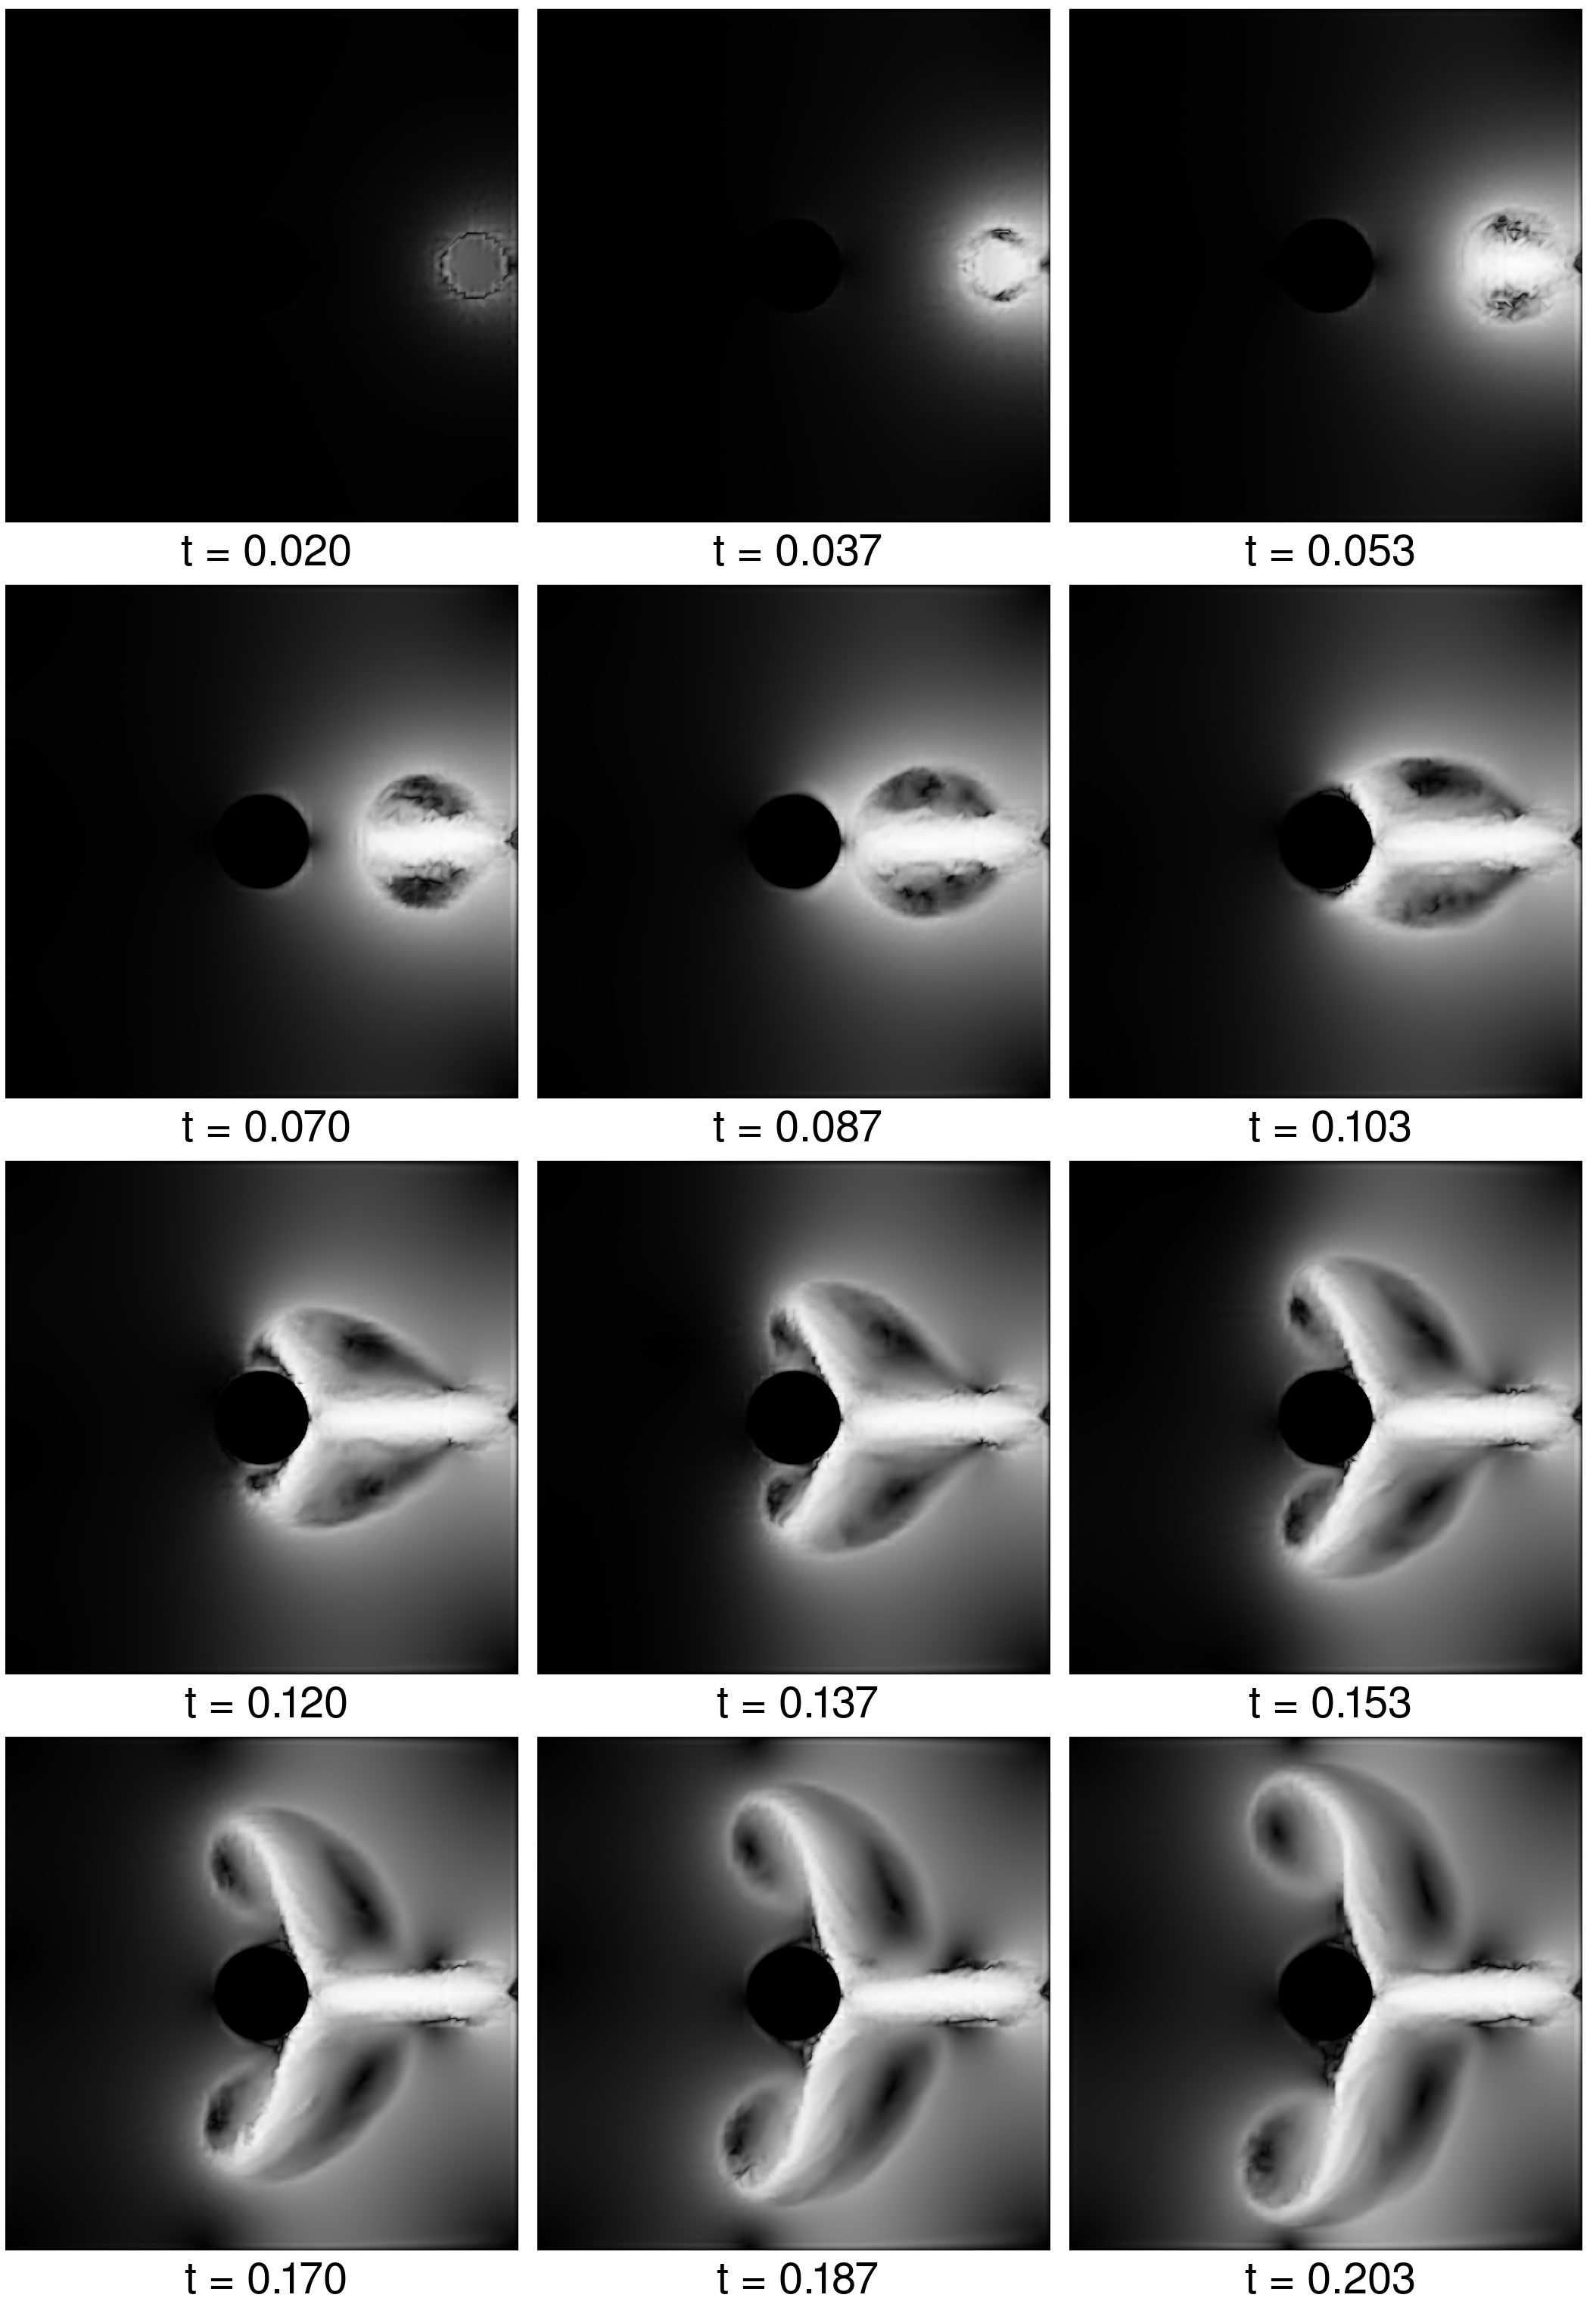
\includegraphics[width=\textwidth]{figures/navier_stokes/navier_0.png}
    \label{fig:navier_0}
\end{figure}
\begin{figure}[htbp]
    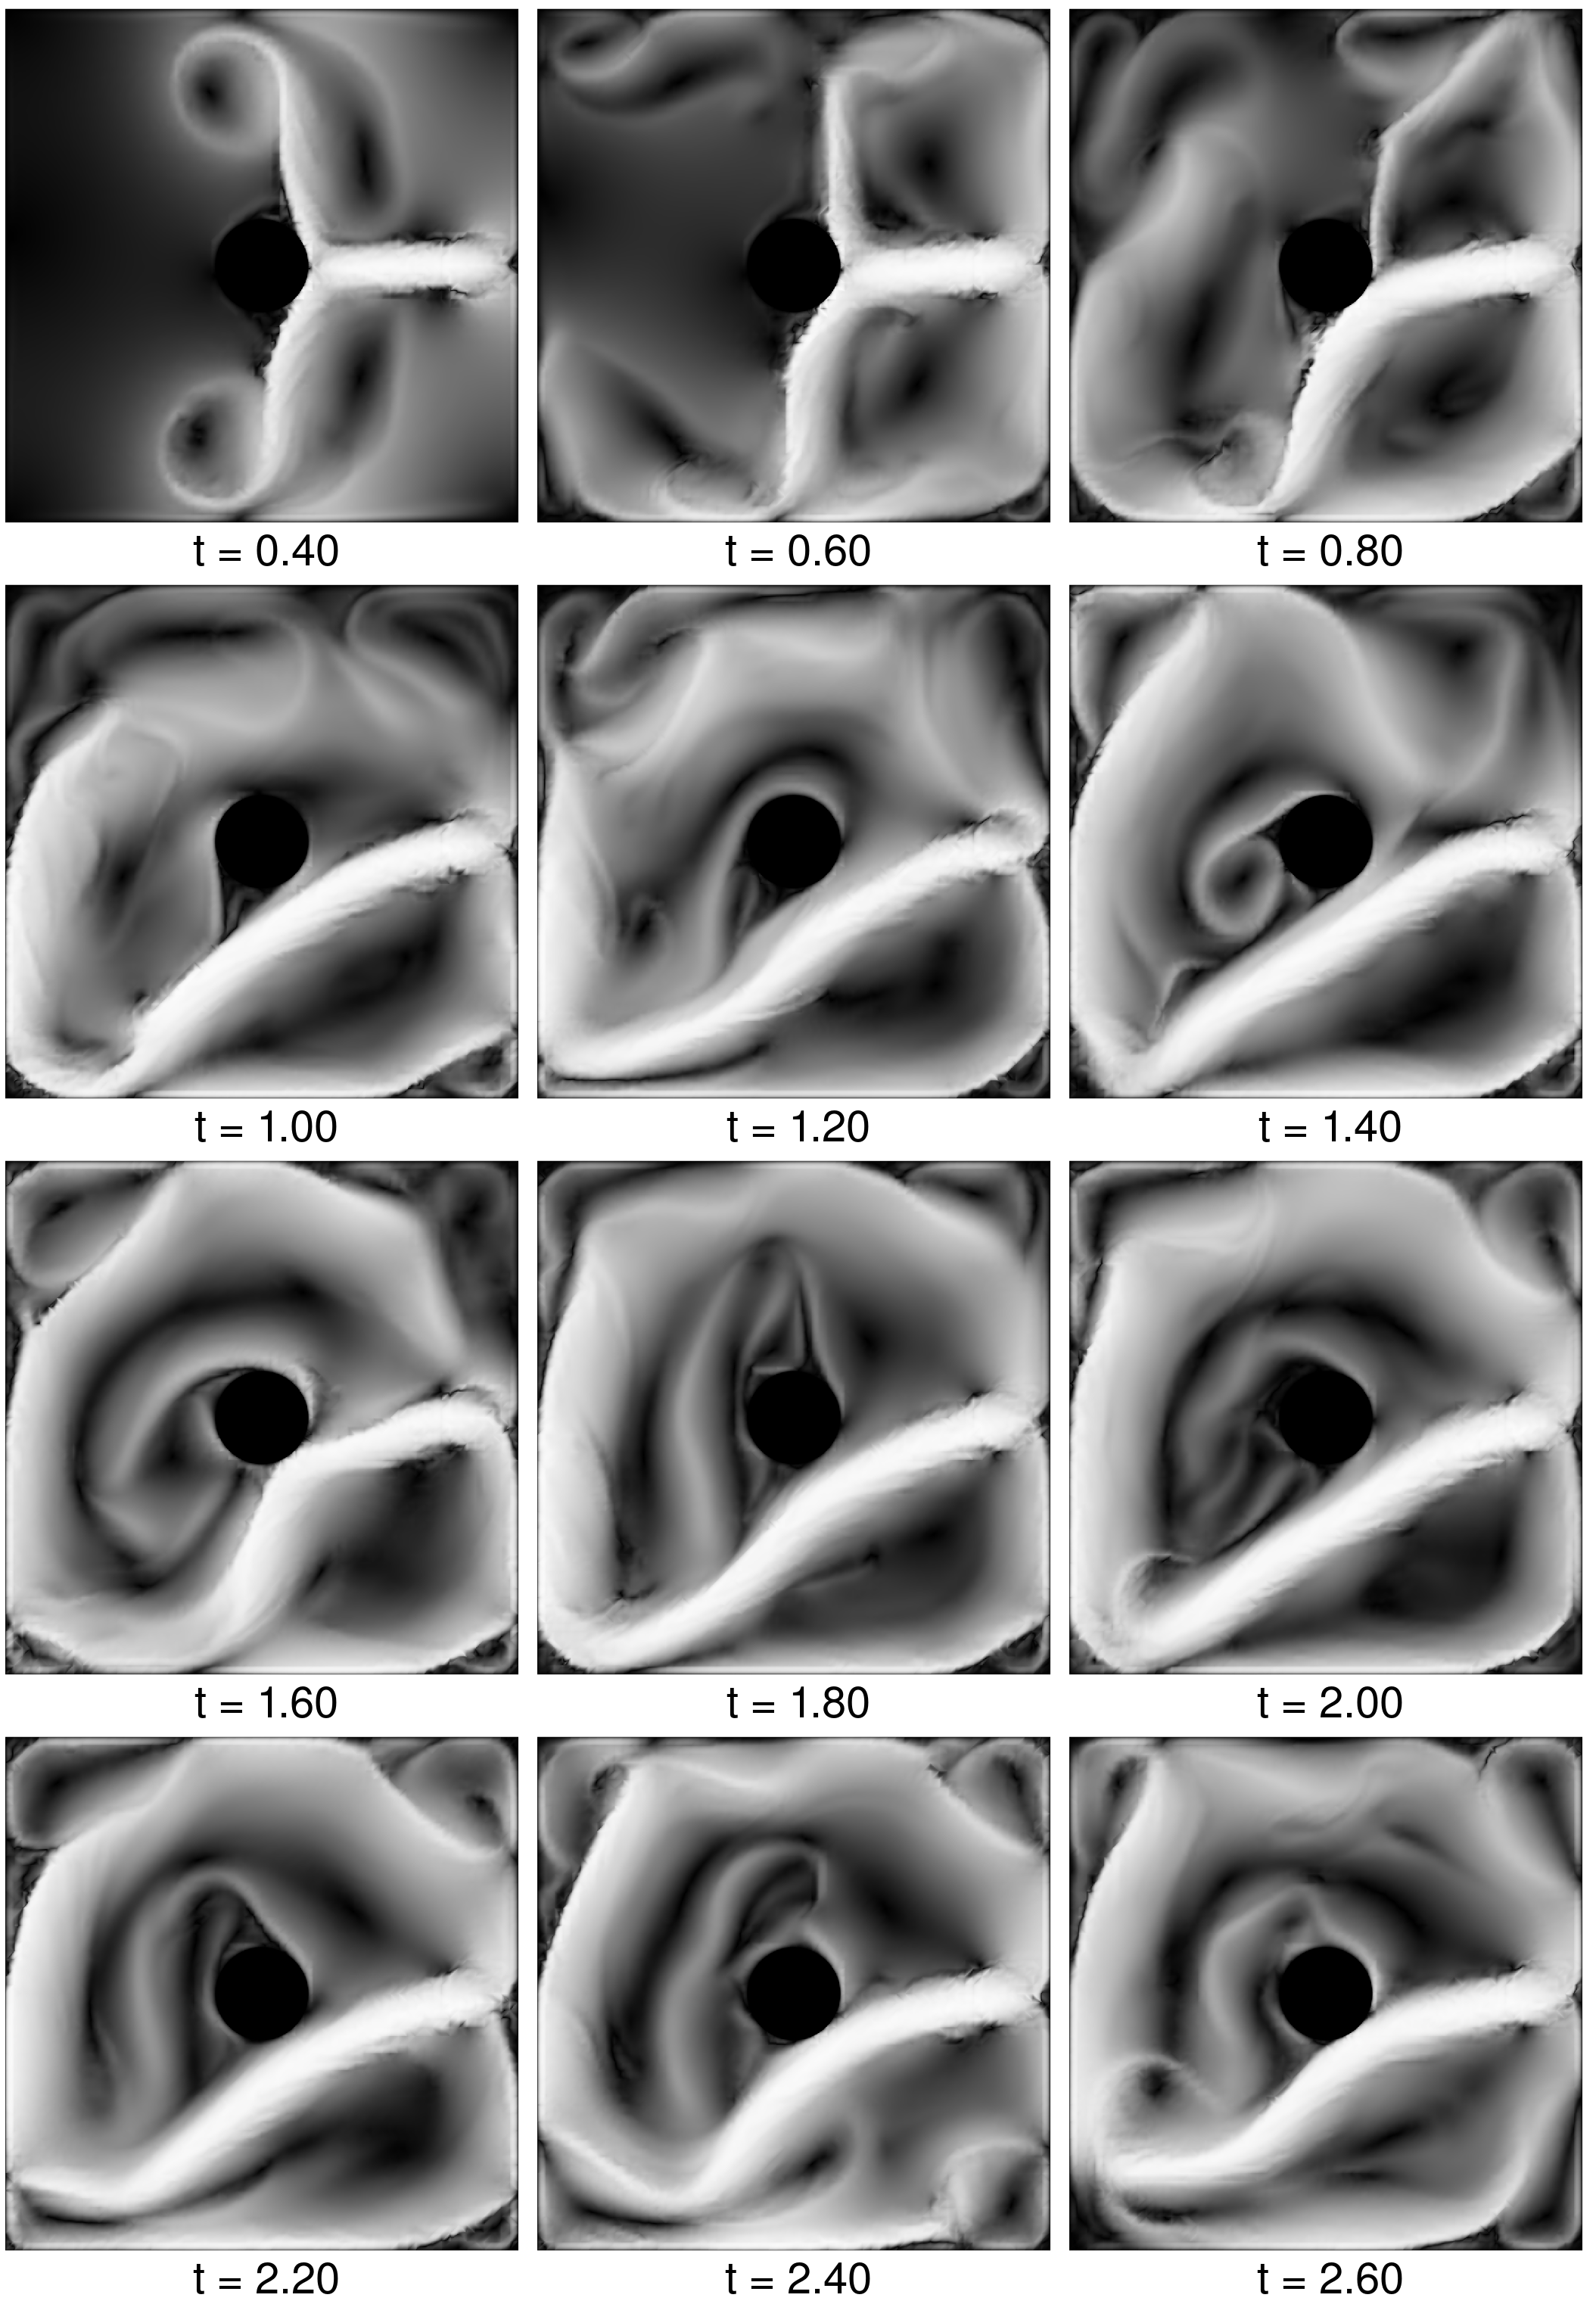
\includegraphics[width=\textwidth]{figures/navier_stokes/navier_1.png}
    \label{fig:navier_1}
\end{figure}

